\chapter{Resultados del estudio}

En este capítulo se recopilan las tablas y gráficas más representativas con los resultados obtenidos en el estudio. Se mostrará una tabla global para cada dimensión, que incluya el error medio obtenido con respecto al óptimo por función y algoritmo, además de una tabla de rankings que ayude a determinar qué algoritmos se comportan mejor en general. Además de las tablas, se incluirán algunas gráficas de convergencia para poder observar de manera más visual qué algoritmos llegan antes a los óptimos y cuáles necesitan de más evaluaciones, así como qué resultados son mejores y en qué proporción con respecto al resto. Por último, se dará una visión analítica acerca de los resultados, dando pie a distintas valoraciones bien fundamentadas que se pueden extraer de las tablas para obtener las conclusiones del estudio. Las tablas y gráficas han sido generadas gracias a la página \textit{TACOLab} \cite{tacolab}.

Para valorar mejor cómo funcionan los algoritmos del estudio, se ha escogido un algoritmo de referencia en el que muchos de ellos están inspirados, y se ha añadido a las tablas de resultados. Se trata de un Particle Swarm Optimization, un algoritmo que ya se describió anteriormente en este documento. Comparar los resultados que arroje este algoritmo con el de aquellos socioinspirados que se comportan de manera similar servirá para determinar si dicha modificación al PSO es significativa o por el contrario no aporta gran cosa. El código para ejecutar el PSO ha sido obtenido de este repositorio de GitHub \cite{pso-github}.

\begin{table}
	\centering
	\resizebox{\textwidth}{!}{
	\begin{tabular}{cccccccc}
		\toprule
		{} &        \textbf{ASO} &         \textbf{IA} &        \textbf{ICA} &        \textbf{POA} &        \textbf{PSO} &        \textbf{SEA} &        \textbf{SLC} \\
		\midrule
		\textbf{F01}  &  5.071e+00 &  1.981e+03 &  6.705e+03 &  1.460e+04 &  2.828e+03 &  1.348e+01 &  \textbf{0.000e+00} \\
		\textbf{F02}  &  1.980e+02 &  3.436e+03 &  9.925e+03 &  1.297e+04 &  1.719e+04 &  1.292e+02 &  \textbf{1.160e-08} \\
		\textbf{F03}  &  1.137e+06 &  9.482e+06 &  5.012e+07 &  1.251e+08 &  9.043e+07 &  5.509e+06 &  \textbf{2.971e+04} \\
		\textbf{F04}  &  6.140e+01 &  4.165e+03 &  1.169e+04 &  1.365e+04 &  7.709e+04 &  9.347e+02 &  \textbf{3.592e-05} \\
		\textbf{F05}  &  8.036e+02 &  7.204e+03 &  8.684e+03 &  1.901e+04 &  1.752e+04 &  6.230e+02 &  \textbf{4.590e-03} \\
		\midrule
		\textbf{F06}  &  1.388e+04 &  6.219e+07 &  9.836e+08 &  3.383e+09 &  3.263e+08 &  2.764e+04 &  \textbf{8.802e+01} \\
		\textbf{F07}  &  5.061e+00 &  1.890e+03 &  1.259e+03 &  3.131e+03 &  2.253e+03 &  1.920e+03 &  \textbf{5.673e-01} \\
		\textbf{F08}  &  2.035e+01 &  2.041e+01 &  2.053e+01 &  2.093e+01 &  2.022e+01 &  2.028e+01 &  \textbf{2.019e+01} \\
		\textbf{F09}  &  \textbf{3.529e+00} &  6.505e+01 &  7.433e+01 &  8.867e+01 &  1.201e+02 &  3.292e+01 &  3.881e+00 \\
		\textbf{F10}  &  9.487e+00 &  9.127e+01 &  9.884e+01 &  1.162e+02 &  2.073e+02 &  2.739e+01 &  \textbf{4.584e+00} \\
		\textbf{F11}  &  7.778e+00 &  9.458e+00 &  1.028e+01 &  1.345e+01 &  7.542e+00 &  8.258e+00 &  \textbf{3.801e+00} \\
		\textbf{F12}  &  1.230e+03 &  2.248e+04 &  5.419e+04 &  1.107e+05 &  5.515e+04 &  2.686e+03 &  \textbf{4.385e+02} \\
		\midrule
		\textbf{F13}  &  \textbf{5.364e-01} &  6.426e+00 &  1.014e+01 &  9.040e+00 &  6.991e+00 &  2.393e+00 &  5.710e-01 \\
		\textbf{F14}  &  3.754e+00 &  3.927e+00 &  4.111e+00 &  4.501e+00 &  4.853e+00 &  3.606e+00 &  \textbf{2.460e+00} \\
		\midrule
		\textbf{F15}  &  \textbf{2.538e+02} &  5.274e+02 &  6.972e+02 &  9.631e+02 &  7.499e+02 &  4.281e+02 &  2.721e+02 \\
		\textbf{F16}  &  1.216e+02 &  2.799e+02 &  3.968e+02 &  6.118e+02 &  5.502e+02 &  1.679e+02 &  \textbf{1.108e+02} \\
		\textbf{F17}  &  5.554e+01 &  1.346e+02 &  8.380e+01 &  1.128e+02 &  2.099e+02 &  9.551e+01 &  \textbf{3.215e+01} \\
		\textbf{F18}  &  \textbf{7.774e+02} &  1.091e+03 &  1.129e+03 &  1.383e+03 &  1.245e+03 &  1.037e+03 &  8.838e+02 \\
		\textbf{F19}  &  \textbf{8.096e+02} &  1.084e+03 &  1.161e+03 &  1.383e+03 &  1.194e+03 &  8.563e+02 &  8.373e+02 \\
		\textbf{F20}  &  \textbf{8.158e+02} &  1.082e+03 &  1.161e+03 &  1.383e+03 &  1.267e+03 &  9.720e+02 &  8.648e+02 \\
		\textbf{F21}  &  7.045e+02 &  1.252e+03 &  1.340e+03 &  1.424e+03 &  1.384e+03 &  8.994e+02 &  \textbf{6.702e+02} \\
		\textbf{F22}  &  7.250e+02 &  9.516e+02 &  1.076e+03 &  1.350e+03 &  1.248e+03 &  8.940e+02 &  \textbf{6.624e+02} \\
		\textbf{F23}  &  9.590e+02 &  1.256e+03 &  1.317e+03 &  1.474e+03 &  1.391e+03 &  1.071e+03 &  \textbf{9.556e+02} \\
		\textbf{F24}  &  \textbf{2.365e+02} &  1.134e+03 &  1.164e+03 &  1.446e+03 &  1.459e+03 &  8.663e+02 &  2.800e+02 \\
		\textbf{F25}  &  \textbf{5.109e+02} &  1.346e+03 &  1.101e+03 &  2.118e+03 &  1.214e+03 &  5.243e+02 &  5.188e+02 \\
		\midrule
		\textbf{Best} &          8 &          0 &          0 &          0 &          0 &          0 &         \textbf{17} \\
		\bottomrule
\end{tabular}}
	\caption{Resultados medios del benchmark CEC2005 para dimensión 10.}\label{t:resultados-10}
\end{table}

\begin{table}
	\centering
	\begin{tabular}{cccccccc}
		\toprule
		{} &    \textbf{ASO} &     \textbf{IA} &    \textbf{ICA} &    \textbf{POA} &    \textbf{PSO} &    \textbf{SEA} &    \textbf{SLC} \\
		\midrule
		\textbf{F01}  &      2 &      4 &      6 &      7 &      5 &      3 &      \textbf{1} \\
		\textbf{F02}  &      3 &      4 &      5 &      6 &      7 &      2 &      \textbf{1} \\
		\textbf{F03}  &      2 &      4 &      5 &      7 &      6 &      3 &      \textbf{1} \\
		\textbf{F04}  &      2 &      4 &      5 &      6 &      7 &      3 &      \textbf{1} \\
		\textbf{F05}  &      3 &      4 &      5 &      7 &      6 &      2 &      \textbf{1} \\
		\midrule
		\textbf{F06}  &      2 &      4 &      6 &      7 &      5 &      3 &      \textbf{1} \\
		\textbf{F07}  &      2 &      4 &      3 &      7 &      6 &      5 &      \textbf{1} \\
		\textbf{F08}  &      4 &      5 &      6 &      7 &      2 &      3 &      \textbf{1} \\
		\textbf{F09}  &      \textbf{1} &      4 &      5 &      6 &      7 &      3 &      2 \\
		\textbf{F10}  &      2 &      4 &      5 &      6 &      7 &      3 &      \textbf{1} \\
		\textbf{F11}  &      3 &      5 &      6 &      7 &      2 &      4 &      \textbf{1} \\
		\textbf{F12}  &      2 &      4 &      5 &      7 &      6 &      3 &      \textbf{1} \\
		\midrule
		\textbf{F13}  &      \textbf{1} &      4 &      7 &      6 &      5 &      3 &      2 \\
		\textbf{F14}  &      3 &      4 &      5 &      6 &      7 &      2 &      \textbf{1} \\
		\midrule
		\textbf{F15}  &      \textbf{1} &      4 &      5 &      7 &      6 &      3 &      2 \\
		\textbf{F16}  &      2 &      4 &      5 &      7 &      6 &      3 &      \textbf{1} \\
		\textbf{F17}  &      2 &      6 &      3 &      5 &      7 &      4 &      \textbf{1} \\
		\textbf{F18}  &      \textbf{1} &      4 &      5 &      7 &      6 &      3 &      2 \\
		\textbf{F19}  &      \textbf{1} &      4 &      5 &      7 &      6 &      3 &      2 \\
		\textbf{F20}  &      \textbf{1} &      4 &      5 &      7 &      6 &      3 &      2 \\
		\textbf{F21}  &      2 &      4 &      5 &      7 &      6 &      3 &      \textbf{1} \\
		\textbf{F22}  &      2 &      4 &      5 &      7 &      6 &      3 &      \textbf{1} \\
		\textbf{F23}  &      2 &      4 &      5 &      7 &      6 &      3 &      \textbf{1} \\
		\textbf{F24}  &      \textbf{1} &      4 &      5 &      6 &      7 &      3 &      2 \\
		\textbf{F25}  &      \textbf{1} &      6 &      4 &      7 &      5 &      3 &      2 \\
		\midrule
		\textbf{Mean} &  1.920 &  4.240 &  5.040 &  6.640 &  5.800 &  3.040 &  \textbf{1.320} \\
		\bottomrule
	\end{tabular}
	\caption{Ranking de resultados del benchmark CEC2005 para dimensión 10.}\label{t:ranking-10}
\end{table}

\begin{table}
	\resizebox{\textwidth}{!}{
	\begin{tabular}{cccccccc}
		\toprule
		{} &        \textbf{ASO} &         \textbf{IA} &        \textbf{ICA} &        \textbf{POA} &        \textbf{PSO} &        \textbf{SEA} &        \textbf{SLC} \\
		\midrule
		\textbf{F01}  &  1.288e+02 &  3.626e+04 &  6.173e+04 &  6.584e+04 &  8.855e+04 &  1.866e+03 &  \textbf{0.000e+00} \\
		\textbf{F02}  &  2.489e+03 &  4.569e+04 &  7.734e+04 &  8.917e+04 &  1.313e+05 &  1.220e+04 &  \textbf{1.179e-02} \\
		\textbf{F03}  &  1.602e+07 &  3.321e+08 &  1.194e+09 &  1.466e+09 &  1.633e+09 &  2.487e+07 &  \textbf{5.643e+05} \\
		\textbf{F04}  &  1.092e+04 &  5.443e+04 &  1.054e+05 &  8.943e+04 &  5.277e+05 &  3.946e+04 &  \textbf{4.680e+00} \\
		\textbf{F05}  &  4.663e+03 &  2.588e+04 &  3.480e+04 &  4.441e+04 &  4.695e+04 &  1.343e+04 &  \textbf{4.157e+03} \\
		\midrule
		\textbf{F06}  &  1.317e+07 &  9.779e+09 &  3.827e+10 &  2.916e+10 &  6.250e+10 &  1.173e+08 &  \textbf{7.574e+02} \\
		\textbf{F07}  &  1.646e+02 &  8.951e+03 &  9.200e+03 &  1.252e+04 &  1.069e+04 &  5.696e+03 &  \textbf{3.926e-01} \\
		\textbf{F08}  &  2.097e+01 &  2.096e+01 &  2.112e+01 &  2.134e+01 &  \textbf{2.064e+01} &  2.082e+01 &  2.090e+01 \\
		\textbf{F09}  &  \textbf{2.940e+01} &  3.278e+02 &  4.076e+02 &  4.047e+02 &  4.455e+02 &  2.046e+02 &  9.910e+01 \\
		\textbf{F10}  &  2.528e+02 &  4.707e+02 &  6.905e+02 &  6.595e+02 &  9.259e+02 &  2.872e+02 &  \textbf{9.004e+01} \\
		\textbf{F11}  &  3.956e+01 &  4.008e+01 &  4.330e+01 &  4.749e+01 &  3.427e+01 &  3.429e+01 &  \textbf{2.410e+01} \\
		\textbf{F12}  &  2.710e+04 &  1.026e+06 &  1.512e+06 &  1.579e+06 &  4.473e+05 &  1.481e+05 &  \textbf{9.489e+03} \\
		\midrule
		\textbf{F13}  &  3.567e+00 &  8.211e+01 &  1.858e+02 &  4.855e+01 &  1.075e+02 &  1.657e+01 &  \textbf{3.425e+00} \\
		\textbf{F14}  &  1.352e+01 &  1.359e+01 &  1.381e+01 &  1.437e+01 &  1.488e+01 &  1.337e+01 &  \textbf{1.207e+01} \\
		\midrule
		\textbf{F15}  &  \textbf{2.950e+02} &  8.825e+02 &  1.049e+03 &  1.200e+03 &  9.587e+02 &  6.849e+02 &  5.160e+02 \\
		\textbf{F16}  &  \textbf{8.460e+01} &  6.003e+02 &  9.486e+02 &  1.191e+03 &  8.238e+02 &  4.667e+02 &  2.964e+02 \\
		\textbf{F17}  &  5.693e+01 &  1.875e+02 &  8.462e+01 &  1.054e+02 &  2.195e+02 &  1.872e+02 &  \textbf{1.831e+01} \\
		\textbf{F18}  &  9.354e+02 &  1.184e+03 &  1.284e+03 &  1.268e+03 &  1.402e+03 &  9.586e+02 &  \textbf{9.107e+02} \\
		\textbf{F19}  &  \textbf{9.170e+02} &  1.178e+03 &  1.283e+03 &  1.261e+03 &  1.367e+03 &  9.666e+02 &  9.192e+02 \\
		\textbf{F20}  &  9.170e+02 &  1.158e+03 &  1.283e+03 &  1.261e+03 &  1.365e+03 &  9.758e+02 &  \textbf{9.094e+02} \\
		\textbf{F21}  &  \textbf{6.006e+02} &  1.325e+03 &  1.412e+03 &  1.386e+03 &  1.419e+03 &  1.066e+03 &  7.375e+02 \\
		\textbf{F22}  &  9.227e+02 &  1.306e+03 &  1.558e+03 &  1.740e+03 &  1.599e+03 &  1.193e+03 &  \textbf{9.108e+02} \\
		\textbf{F23}  &  9.780e+02 &  1.323e+03 &  1.383e+03 &  1.385e+03 &  1.422e+03 &  1.211e+03 &  \textbf{9.097e+02} \\
		\textbf{F24}  &  \textbf{2.021e+02} &  1.367e+03 &  1.468e+03 &  1.464e+03 &  1.602e+03 &  1.220e+03 &  9.086e+02 \\
		\textbf{F25}  &  \textbf{3.574e+02} &  1.410e+03 &  1.746e+03 &  1.978e+03 &  1.563e+03 &  9.508e+02 &  3.995e+02 \\
		\midrule
		\textbf{Best} &          7 &          0 &          0 &          0 &          1 &          0 &         \textbf{17} \\
		\bottomrule
\end{tabular}}
	\caption{Resultados medios del benchmark CEC2005 para dimensión 30.}\label{t:resultados-30}
\end{table}

\begin{table}
	\centering
	\begin{tabular}{cccccccc}
		\toprule
		{} &    \textbf{ASO} &     \textbf{IA} &    \textbf{ICA} &    \textbf{POA} &    \textbf{PSO} &    \textbf{SEA} &    \textbf{SLC} \\
		\midrule
		\textbf{F01}  &      2 &      4 &      5 &      6 &      7 &      3 &      \textbf{1} \\
		\textbf{F02}  &      2 &      4 &      5 &      6 &      7 &      3 &      \textbf{1} \\
		\textbf{F03}  &      2 &      4 &      5 &      6 &      7 &      3 &      \textbf{1} \\
		\textbf{F04}  &      2 &      4 &      6 &      5 &      7 &      3 &      \textbf{1} \\
		\textbf{F05}  &      2 &      4 &      5 &      6 &      7 &      3 &      \textbf{1} \\
		\midrule
		\textbf{F06}  &      2 &      4 &      6 &      5 &      7 &      3 &      \textbf{1} \\
		\textbf{F07}  &      2 &      4 &      5 &      7 &      6 &      3 &      \textbf{1} \\
		\textbf{F08}  &      5 &      4 &      6 &      7 &      \textbf{1} &      2 &      3 \\
		\textbf{F09}  &      \textbf{1} &      4 &      6 &      5 &      7 &      3 &      2 \\
		\textbf{F10}  &      2 &      4 &      6 &      5 &      7 &      3 &      \textbf{1} \\
		\textbf{F11}  &      4 &      5 &      6 &      7 &      2 &      3 &      \textbf{1} \\
		\textbf{F12}  &      2 &      5 &      6 &      7 &      4 &      3 &      \textbf{1} \\
		\midrule
		\textbf{F13}  &      2 &      5 &      7 &      4 &      6 &      3 &      \textbf{1} \\
		\textbf{F14}  &      3 &      4 &      5 &      6 &      7 &      2 &      \textbf{1} \\
		\midrule
		\textbf{F15}  &      \textbf{1} &      4 &      6 &      7 &      5 &      3 &      2 \\
		\textbf{F16}  &      \textbf{1} &      4 &      6 &      7 &      5 &      3 &      2 \\
		\textbf{F17}  &      2 &      6 &      3 &      4 &      7 &      5 &      \textbf{1} \\
		\textbf{F18}  &      2 &      4 &      6 &      5 &      7 &      3 &      \textbf{1} \\
		\textbf{F19}  &      \textbf{1} &      4 &      6 &      5 &      7 &      3 &      2 \\
		\textbf{F20}  &      2 &      4 &      6 &      5 &      7 &      3 &      \textbf{1} \\
		\textbf{F21}  &      \textbf{1} &      4 &      6 &      5 &      7 &      3 &      2 \\
		\textbf{F22}  &      2 &      4 &      5 &      7 &      6 &      3 &      \textbf{1} \\
		\textbf{F23}  &      2 &      4 &      5 &      6 &      7 &      3 &      \textbf{1} \\
		\textbf{F24}  &      \textbf{1} &      4 &      6 &      5 &      7 &      3 &      2 \\
		\textbf{F25}  &      \textbf{1} &      4 &      6 &      7 &      5 &      3 &      2 \\
		\textbf{Mean} &  1.960 &  4.200 &  5.600 &  5.800 &  6.080 &  3.000 &  \textbf{1.360} \\
		\bottomrule
	\end{tabular}
	\caption{Ranking de resultados del benchmark CEC2005 para dimensión 30.}\label{t:ranking-30}
\end{table}

\begin{table}
	\centering
	\begin{tabular}{lrr}
		\toprule
		{} &  \textbf{D-10} &  \textbf{D-30} \\
		\midrule
		\textbf{ASO} &   8 &   7 \\
		\textbf{IA}  &   0 &   0 \\
		\textbf{ICA} &   0 &   0 \\
		\textbf{POA} &   0 &   0 \\
		\textbf{PSO} &   0 &   1 \\
		\textbf{SEA} &   0 &   0 \\
		\textbf{SLC} &  \textbf{17} &  \textbf{17} \\
		\bottomrule
	\end{tabular}
	\caption{Mejores soluciones de cada algoritmo para cada dimensión.}\label{t:best-global}
\end{table}

\begin{table}
	\centering
	\begin{tabular}{lrr}
		\toprule
		{} &    \textbf{D-10} &    \textbf{D-30} \\
		\midrule
		\textbf{ASO} &  1.92 &  1.96 \\
		\textbf{IA}  &  4.24 &  4.20 \\
		\textbf{ICA} &  5.04 &  5.60 \\
		\textbf{POA} &  6.64 &  5.80 \\
		\textbf{PSO} &  5.80 &  6.08 \\
		\textbf{SEA} &  3.04 &  3.00 \\
		\textbf{SLC} &  \textbf{1.32} &  \textbf{1.36} \\
		\bottomrule
	\end{tabular}
	\caption{Ranking global de cada algoritmo para cada dimensión.}\label{t:ranking-global}
\end{table}

\begin{figure}
	\centering
	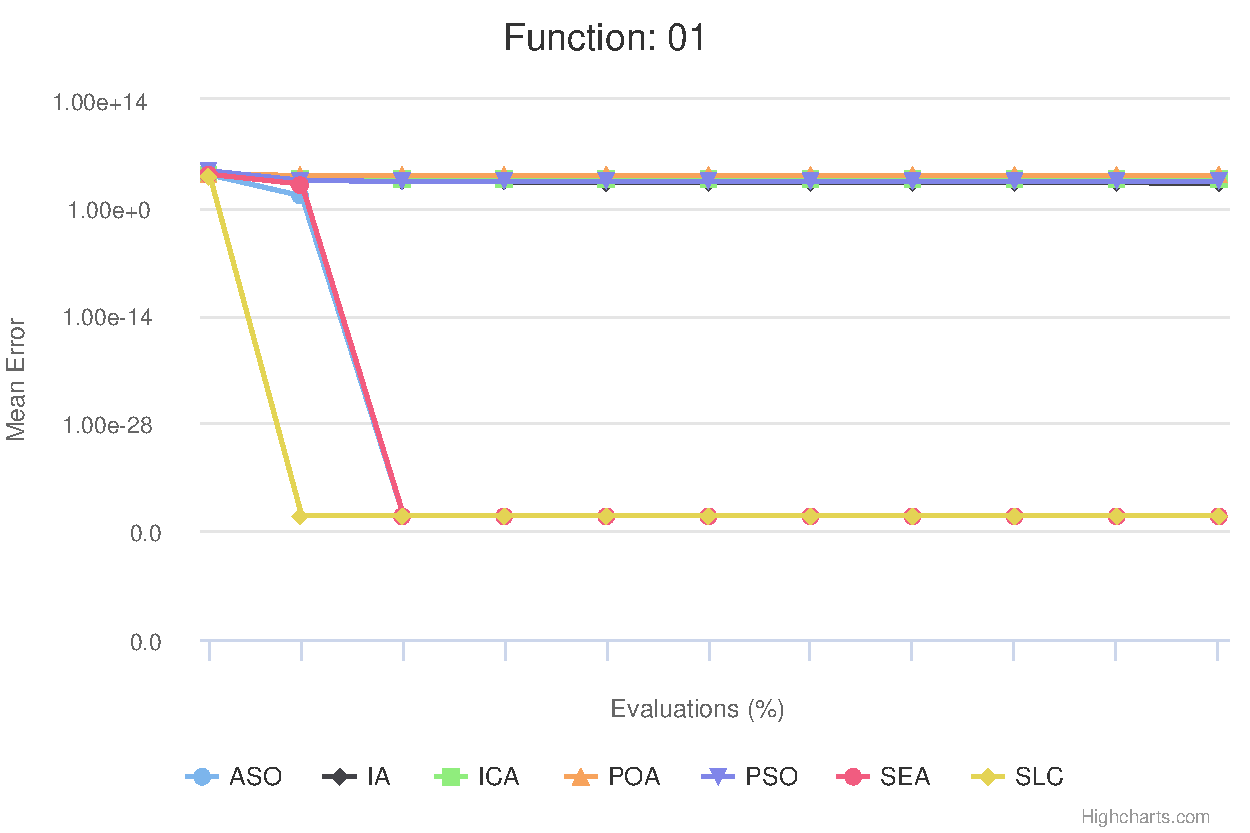
\includegraphics[scale=0.6]{imagenes/grafica-convergencia-10-1.pdf}
	\caption{Gráfica de convergencia de la función 1 para dimensión 10.}
	\label{grafica-convergencia-10-1}
\end{figure}

\begin{figure}
	\centering
	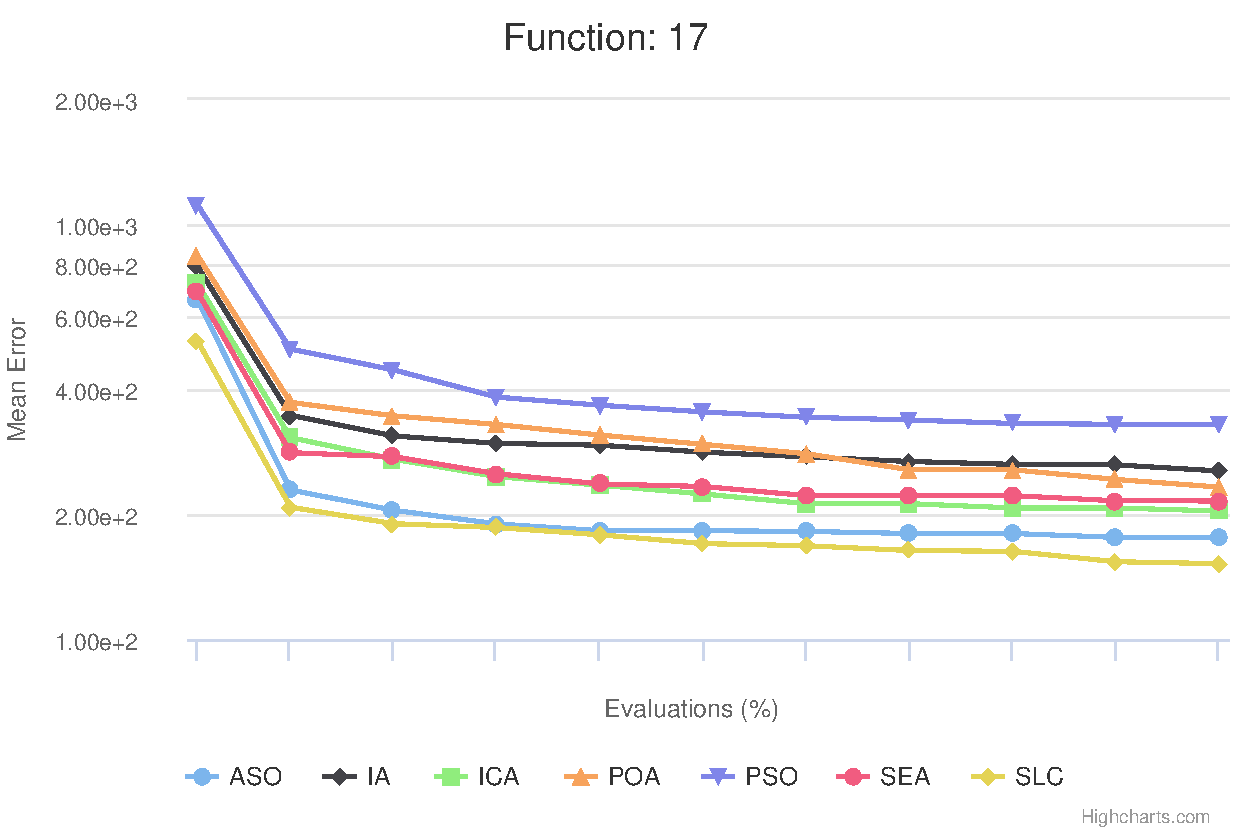
\includegraphics[scale=0.6]{imagenes/grafica-convergencia-10-17.pdf}
	\caption{Gráfica de convergencia de la función 17 para dimensión 10.}
	\label{grafica-convergencia-10-17}
\end{figure}

\begin{figure}
	\centering
	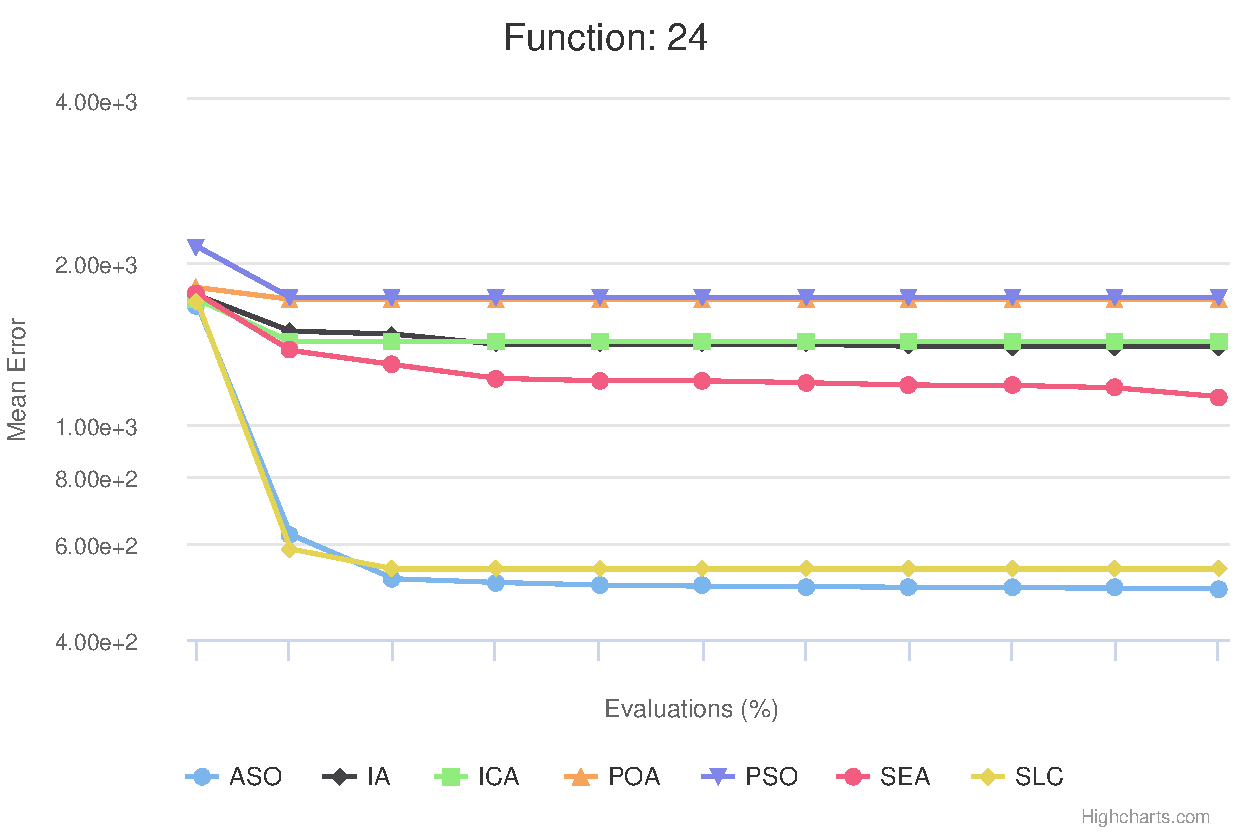
\includegraphics[scale=0.6]{imagenes/grafica-convergencia-10-24.pdf}
	\caption{Gráfica de convergencia de la función 24 para dimensión 10.}
	\label{grafica-convergencia-10-24}
\end{figure}

En primer lugar se van a analizar los resultados para la dimensión 10. Para ello conviene fijarse en la tabla \ref{t:resultados-10} que contiene el error medio con respecto al óptimo obtenido por cada algoritmo a lo largo de 10 ejecuciones sobre una misma función en dicha dimensión. Con un simple vistazo a la tabla se puede observar que en general en las funciones unimodales (desde F1 hasta F5) los algoritmos dan resultados muy malos, en especial PSO, el algoritmo de referencia. Y es que para estas funciones la mayoría de los algoritmos mejoran su resultado, salvo el POA que obtiene errores aún mayores.

Con respecto al POA, fijándose en la tabla \ref{t:ranking-10} se puede observar que únicamente en 8 de las 25 funciones no acaba en última posición. Por tanto, hay un total de 17 funciones en las que no consigue vencer ni al algoritmo de referencia en el que se basa, un resultado que resulta muy poco favorecedor. Se puede afirmar que POA es el peor algoritmo para cada grupo de funciones en dimensión 10.

Yendo al extremo contrario, a los que mejor se comportan en estas funciones unimodales, se encuentran ASO y SLC. Esto se puede observar tanto en la tabla \ref{t:resultados-10} en la que se aprecia que sus errores son varios órdenes de magnitud menores que los del resto, y en las gráficas de convergencia como la de la figura \ref{grafica-convergencia-10-1}, donde aparte de verse la diferencia en cuanto a ajuste de la solución destaca la rápida convergencia de estos algoritmos.

SLC es el mejor en unimodales, llegando o acariciando el óptimo en dos de ellas, y siendo en todo momento sus errores varios órdenes de magnitud inferiores a los del resto, a excepción de ASO en algunos casos. SLC también destaca con algunas de las mejores soluciones para las multimodales básicas, y aunque para las híbridas también funciona bien y se mantiene en un más que correcto segundo lugar, ASO es el algoritmo que mejores resultados da en ese campo.

Se puede decir que ambos algoritmos van casi de la mano en multimodales, ya que aunque el ASO explota sus ventajas cuanta más compleja sea la función, también es cierto que SLC obtiene muy buenos resultados para funciones con ruido, como son en este caso F4 y F17. Es curioso el caso de este algoritmo ya que maneja tan bien el ruido que para la misma función encuentra una mejor solución con ruido (F17) que sin él (F16).

Si se estudia la complejidad y el relieve del espacio de búsqueda de las funciones, se puede afirmar que SLC funciona especialmente bien en aquellas funciones con relieve suave (F1, F2) mientras que ASO lo hace para las que tienen un relieve más tortuoso y con más óptimos locales (F9, F18, F19). También SLC funciona bien con las que están rotadas, como F7, F8, F10 o F11. En este tipo de funciones los algoritmos basados en PSO sufren, ya que PSO es menos robusto frente a rotaciones que un Differential Evolution, por ejemplo.

Con respecto al resto de algoritmos que se encuentran en una posición intermedia, al menos se puede valorar que mejoran al algoritmo de referencia PSO en casi todas las funciones. En el caso del ICA, las diferencias no son muy significativas pero sin embargo sí que obtiene un error menor que PSO de manera generalizada, exceptuando F8 y F11 donde PSO destaca, siendo sólo superado por SLC. Si se valora en las funciones híbridas, sí que se puede encontrar una tendencia clara de mejora, y es que es sistemáticamente mejor para aquellas funciones entre F15 y F25. Este dato se puede apreciar de manera menos confusa en la tabla \ref{t:ranking-10}, comprobando que la columna de ICA es siempre menos que la de PSO a partir de dichas funciones.

SEA es el tercer algoritmo que mejores resultados encuentra de manera general, de acuerdo a la tabla de ranking \ref{t:ranking-10}. Sin embargo, como se puede observar en la gráfica de convergencia de la función 24 (figura \ref{grafica-convergencia-10-24}) la distancia entre las soluciones de los algoritmos ASO y SLC y la del SEA es muy grande. A pesar de ser el tercer mejor algoritmo y destacar sobre los otros 4, está a bastante de acercarse a SLC y ASO. Esto puede observarse para casi todas las funciones si se compara en la tabla \ref{t:resultados-10} la columna de SEA con las de estos algoritmos. Con respecto a IA ocurre una situación parecida, resultando mejor que ICA, POA y PSO pero encontrándose lejos de SEA, que a su vez lo está de los algoritmos líderes del estudio.

Si se estudian los distintos grupos de algoritmos en función a su relación con PSO, se pueden sacar conclusiones interesantes. ICA y POA son los que más se asemejan a este algoritmo, en los que su mayor innovación consiste realmente en manejar varias estructuras similares a un PSO dentro del propio problema, y hacer que interactúen entre ellas. Sin embargo su interacción es bastante pobre, y la exploración se puede ver que no es nada del otro mundo con respecto al algoritmo original, como puede observarse en la gráfica de la figura \ref{grafica-convergencia-10-1}. IA es similar a POA pero con una interacción más compleja entre sus soluciones, lo que se puede ver reflejado en las tablas que supone un margen de mejora amplio entre ambas técnicas. SEA y ASO implementan un componente histórico que ayuda a mejorar las soluciones, ya que además viene acompañado en ambos casos de una toma de decisiones basada en el estado temporal del problema. Dicha bifurcación en el camino del individuo parece estar mejor planteada en ASO, que consigue los mejores resultados de los algoritmos que parten de una idea basada en PSO, y es que SLC, el algoritmo que indiscutiblemente encuentra mejores resultados generales, es un algoritmo similar a Differential Evolution que utiliza mutaciones. Sus fundamentos básicos, algo distintos a los del resto de socioinspirados que se han estudiado, permiten que destaque sobre el resto y llegue a alcanzar esas soluciones tan positivas en la mayoría de los casos.

En dimensión 30 los resultados siguen una ruta similar, como se puede valorar comparando en la tabla \ref{t:ranking-global} las columnas correspondientes a dimensión 10 y 30 para cada algoritmo. Se observa que los valores medios de ranking para cada algoritmo son muy parecidos, solamente cambiando de situación POA, que ahora sí mejora a PSO. En particular, se nota la mejora en todas las unimodales y en bastantes funciones complejas (ver tabla \ref{t:resultados-30}).

El resto de algoritmos sigue una evolución similar. IA, ICA y SEA mantienen un ranking similar, sin destacar en ninguna faceta especial pero siendo al menos constantes en sus ejecuciones si aumenta la dimensionalidad. Lo interesante de esta dimensión se halla en la particular competición que mantienen SLC y ASO. Si en dimensión 10 se citaba la mejora de ASO en funciones multimodales a medida que avanzaba la complejidad, en esta nueva tabla con dimensionalidad 30 puede apreciarse una tendencia hacia lo mismo, que se procede a explicar.

Si se observan detenidamente los resultados de las funciones híbridas en la tabla \ref{t:resultados-30} y se comparan los de ASO y los de SLC, se puede encontraar una pauta curiosa que refuerza la idea presentada en el párrafo anterior. En aquellas funciones en las que SLC es mejor, la distancia entre dicha solución y la que aporta ASO es muy pequeña; sin embargo, si es ASO el algoritmo que mejor resultado aporta, la solución del SLC se encuentra bastante más alejada. Es decir, la diferencia que justificaba que ASO cumplía mejor con las funciones más complejas se acentúa en mayor dimensión, y esto revela que ASO gestiona mejor la diversidad en su espacio de búsqueda.

Como conclusión final a este análisis, puede dar la sensación de que \textbf{SLC}, que es el que más destaca, es un algoritmo que podría formar parte de alguna competición en un CEC. Sin embargo, los resultados aún quedan muy lejos del óptimo para la mayoría de las funciones. Por hacer un símil, se compararán estos resultados del SLC con los aportados por un algoritmo memético que fue presentado en 2008 \cite{memetic-conference} y que comparaba con este mismo benchmark.

Como se observa en la tabla \ref{t:comparativa-slc}, donde se comparan para dimensión 30 todas las funciones multimodales del benchmark de 2005, un total de 20, solamente hay 2 en las que SLC resulte ser mejor. Cabe recordar que SLC es una técnica que vio la luz en 2014 y estos resultados comparativos fueron presentados en 2008, y ya están más que superados por nuevas propuestas. Así que, desde un punto de vista crítico, se debe afirmar que ni siquiera el mejor de los socioinspirados supone un digno rival para algoritmos de hace 10 años.

\begin{table}
	\centering
	\begin{tabular}{ccc}
		\toprule
		{} & \textbf{MA-LSCh-CMA} &        \textbf{SLC} \\
		\midrule
		\textbf{F06}  &   \textbf{1.191e+01} &  7.574e+02 \\
		\textbf{F07}  &   \textbf{8.871e-04} &  3.926e-01 \\
		\textbf{F08}  &   \textbf{2.027e+01} &  2.090e+01 \\
		\textbf{F09}  &   \textbf{7.800e-09} &  9.910e+01 \\
		\textbf{F10}  &   \textbf{1.839e+01} &  9.004e+01 \\
		\textbf{F11}  &   \textbf{4.351e+00} &  2.410e+01 \\
		\textbf{F12}  &   \textbf{7.690e+02} &  9.489e+03 \\
		\textbf{F13}  &   \textbf{2.345e+00} &  3.425e+00 \\
		\textbf{F14}  &   1.268e+01 &  \textbf{1.207e+01} \\
		\textbf{F15}  &   \textbf{3.080e+02} &  5.160e+02 \\
		\textbf{F16}  &   \textbf{1.363e+02} &  2.964e+02 \\
		\textbf{F17}  &   1.346e+02 &  \textbf{1.831e+01} \\
		\textbf{F18}  &   \textbf{8.157e+02} &  9.107e+02 \\
		\textbf{F19}  &   \textbf{8.164e+02} &  9.192e+02 \\
		\textbf{F20}  &   \textbf{8.158e+02} &  9.094e+02 \\
		\textbf{F21}  &   \textbf{5.120e+02} &  7.375e+02 \\
		\textbf{F22}  &   \textbf{5.258e+02} &  9.108e+02 \\
		\textbf{F23}  &   \textbf{5.342e+02} &  9.097e+02 \\
		\textbf{F24}  &   \textbf{2.000e+02} &  9.086e+02 \\
		\textbf{F25}  &   \textbf{2.108e+02} &  3.995e+02 \\
		\midrule
		\textbf{Best} &          \textbf{18} &          2 \\
		\bottomrule
	\end{tabular}
	\caption{Comparativa de funciones multimodales entre SLC y MA-LSCh-CMA.}\label{t:comparativa-slc}
\end{table}